\section{eo\-Atom\-Exchange$<$ Atom $>$ Class Template Reference}
\label{classeo_atom_exchange}\index{eoAtomExchange@{eoAtomExchange}}
A helper class for choosing which genes to exchange.  


{\tt \#include $<$eo\-Variable\-Length\-Crossover.h$>$}

Inheritance diagram for eo\-Atom\-Exchange$<$ Atom $>$::\begin{figure}[H]
\begin{center}
\leavevmode
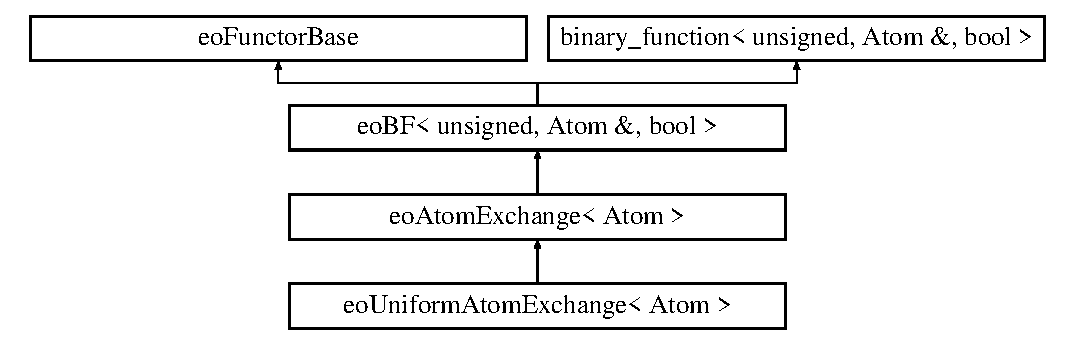
\includegraphics[height=4cm]{classeo_atom_exchange}
\end{center}
\end{figure}
\subsection*{Public Member Functions}
\begin{CompactItemize}
\item 
virtual void {\bf randomize} (unsigned int, unsigned int)\label{classeo_atom_exchange_a0}

\begin{CompactList}\small\item\em a function to initlialize - to be called before every crossover \item\end{CompactList}\item 
virtual std::string {\bf class\-Name} () const =0\label{classeo_atom_exchange_a1}

\begin{CompactList}\small\item\em the inherited {\bf class\-Name()}{\rm (p.\,\pageref{classeo_atom_exchange_a1})} \item\end{CompactList}\end{CompactItemize}


\subsection{Detailed Description}
\subsubsection*{template$<$class Atom$>$ class eo\-Atom\-Exchange$<$ Atom $>$}

A helper class for choosing which genes to exchange. 



Definition at line 41 of file eo\-Variable\-Length\-Crossover.h.

The documentation for this class was generated from the following file:\begin{CompactItemize}
\item 
eo\-Variable\-Length\-Crossover.h\end{CompactItemize}
